\section{Overview and Motivation (Conclusions and Future Work)}\label{sec:c10s1}
\lipsum[129-129]

This section builds on the material in \cref{ch:10}, \cref{ch:1} and the prior work of \citet{main-6}; see also \citep{main-16,main-21}.

\begin{equation}\label{eq:c10s1-a}
  \frac{\partial u}{\partial t} = \nabla\cdot\bigl(D(\mathbf{x})\nabla u\bigr) + f(u),\qquad u(\mathbf{x},0)=u_0(\mathbf{x}).
\end{equation}
Discretising in space with $N$ degrees of freedom yields the semi-discrete system
\begin{align}\label{eq:c10s1-b}
  \mathbf{M}\dot{\mathbf{u}} &= -\mathbf{K}\mathbf{u} + \mathbf{F}(\mathbf{u}),\\
  \mathbf{u}(0) &= \mathbf{u}_0 \in \mathbb{R}^{N}.
\end{align}

Equations~\eqref{eq:c10s1-a} and~\eqref{eq:c10s1-b} are used throughout the remainder of this section.

\lipsum[128-129]

\subsection{Quantitative behaviour}\label{sec:c10s1-q}
Results are collected in \cref{tab:c10s1} and visualised in \cref{fig:c10s1-f1}. Similar trends were reported in~\citep{main-17,main-8}.

\begin{table}[htbp]
\centering
\caption{Summary of measured quantities for experiment set \texttt{c10s1}.}\label{tab:c10s1}
\begin{tabular}{lrrr}
\toprule
Method & Score & Latency & Error \\
\midrule
Alpha & \num{36.8} & \SI{5.73}{\milli\second} & \num{1.050e-4} \\
Beta & \num{33.2} & \SI{1.83}{\milli\second} & \num{4.712e-2} \\
Gamma & \num{69.5} & \SI{1.80}{\milli\second} & \num{1.019e-4} \\
Delta & \num{56.5} & \SI{0.24}{\milli\second} & \num{4.679e-5} \\
Epsilon & \num{92.3} & \SI{5.73}{\milli\second} & \num{3.837e-1} \\
\bottomrule
\end{tabular}
\end{table}

\begin{figure}[htbp]
\centering
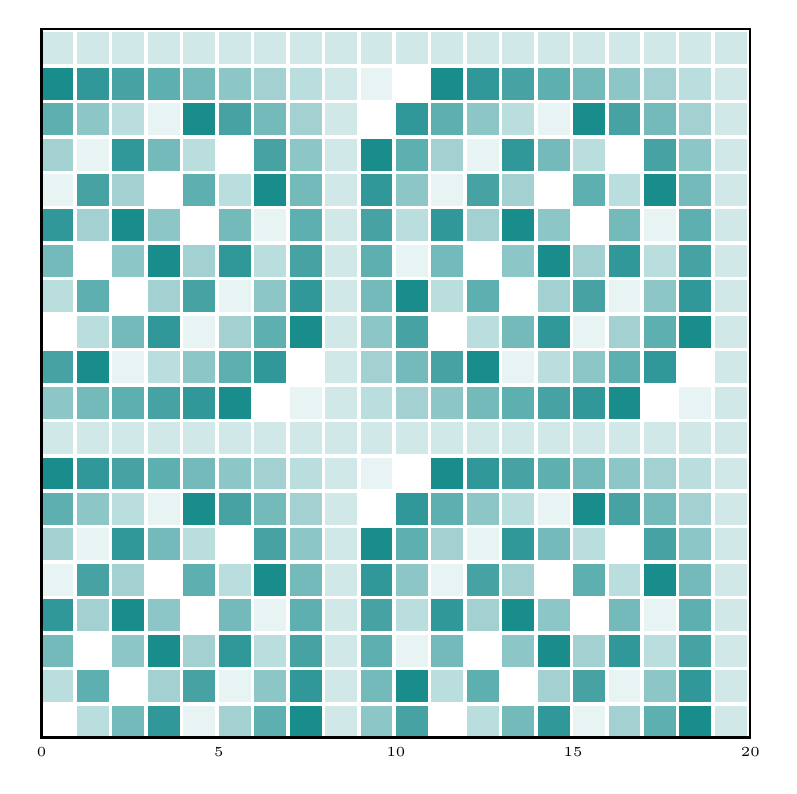
\begin{tikzpicture}[x=4.5mm,y=4.5mm]
\foreach \i in {0,...,19}{\foreach \j in {0,...,19}{\pgfmathtruncatemacro{\v}{mod(\i*3+\j*3+\i*\j,11)*9}
\fill[teal!\v!white](\i,\j)rectangle++(0.9,0.9);}}
\draw[thick](0,0)rectangle(20,20);
\foreach \i in {0,5,...,20}\node[below,font=\tiny]at(\i,0){\i};
\end{tikzpicture}
\caption{Generated figure for \texttt{c10s1-f1} (parameters $a=3$, $b=3$).}\label{fig:c10s1-f1}
\end{figure}

\lipsum[102-103]

\subsection{Implementation notes}\label{sec:c10s1-i}
The core routine is shown in \cref{lst:c10s1}; its complexity is $\mathcal{O}(N\log N)$ per iteration~\cite{main-14}.

\begin{lstlisting}[language=c,caption={Reference implementation for c10s1.},label={lst:c10s1}]
#include <stdio.h>

/* Compute a dot product of two vectors. */
double dot(const double *a, const double *b, int n) {
    double s = 0.0;
    for (int i = 0; i < n; ++i)
        s += a[i] * b[i];
    return s;
}
\end{lstlisting}

\lipsum[88-88]
\begin{theorem}\label{thm:c10s1}
Let $A\in\mathbb{R}^{n\times n}$ be symmetric positive definite with condition number $\kappa$. Then the iteration converges and
$\lVert e_k\rVert_A \le 2\bigl(\tfrac{\sqrt\kappa-1}{\sqrt\kappa+1}\bigr)^k\lVert e_0\rVert_A$.
\end{theorem}
\begin{enumerate}[label=(\roman*)]
\item the bound in \cref{thm:c10s1} is sharp for some initial errors;
\item the constant $2$ cannot be improved in general;
\item preconditioning reduces the effective $\kappa$.
\end{enumerate}

\lipsum[9-9]
